\documentclass[english, 12pt, a4paper]{article}
\usepackage[utf8]{inputenc} 
\usepackage[T1]{fontenc,url} %url
\urlstyle{sf} %sf
\usepackage[toc,page]{appendix}
\usepackage{babel,textcomp,csquotes,ifikompendiumforside, varioref,graphicx, gensymb}
\usepackage[]{circuitikz}
\usepackage{tikz}
\usetikzlibrary{shapes,arrows}
\usepackage[backend=biber,style=numeric-comp, sortcites]{biblatex} 
\usepackage{pgfplots}

\bibliography{ref.bib}

% --------------------------------------------------
\title{ \huge{Successive Approximation Register Analog-to-Digital Converter}}
% \subtitle{Legg til en subtitle dersom det trengs}
\author{By Espen Klein Nilsen\\ and Vegard Midtbøen}
% --------------------------------------------------

 


\begin{document}
\ififorside{}
% \frontmatter{}
\maketitle{} \newpage

\tableofcontents{} \newpage
\listoffigures{} 
\listoftables{} \newpage


%-----------Introduksjon-----
% \mainmatter{}        

\section{Introduction} 
Successive Approximation Register (SAR) Analog-to-Digital Converter (ADC) is a common arctitecture whent talking about Analog-to-Digital (A/D) conversion. A/D conversion is used in almost every
circuits today, and the purpose is to convert a signal from the analig to the digital domain. This is of great interest, because digital signals propagates more efficiently than analog singlals in a 
circuit. By using digital signals, it is easier for the electronic circuit to distinguish from noise \cite{basic-adc}.\\
\\
This task, is as mentrioned, to design a SAR ADC. A block diagram of the system arcitecture is shown in Fig. \ref{block_diagram}. The system includes a sample and hold, a comparator, digital-to-analog 
converter (DAC) and a logic block. The task was to design all this blocks, exept the logic block. The solution for each blocks are discussed in detail in the next chapters.  

\tikzstyle{block} = [draw, fill=blue!20, rectangle, 
    minimum height=4em, minimum width=3em]
\tikzstyle{input} = [coordinate]
\tikzstyle{output} = [coordinate]
\tikzstyle{pinstyle} = [pin edge={to-,thin,black}]
\begin{figure}[!ht]
  \begin{tikzpicture}[auto, node distance=2cm,>=latex']
      % We start by placing the blocks
      \node [input, name=input] {};
      \node [block, right of=input, node distance=2cm] (sample_and_hold) {S\&H};
      \node [block, right of=sample_and_hold, node distance=4cm] (comparator) {Comparator};
      \node [block, right of=comparator, node distance=4cm] (sar_logic) {SAR Logic};
      
      % We draw an edge between the controller and system block to 
      % calculate the coordinate xsh(t). We need it to place the measurement block. 
      \draw [->] (sample_and_hold) -- node[name=xsh(t)] {$x_{sh}(t)$} (comparator);
      \draw [->] (comparator) -- node[name=xc(nT)] {$x_{c}(nT)$} (sar_logic);
      \node [block, below of=sar_logic, node distance=3cm] (dac){DAC};
      \node [output, right of=sar_logic, node distance=3cm] (output) {};
    
      % Once the nodes are placed, connecting them is easy. 
      \draw [draw,->] (input) -- node [name=xc(t)] {$x_{c}(t)$}(sample_and_hold);
      \draw [->] (sar_logic) -- node [name=digital_out] {Digital out}(output);
      \draw [->] (sar_logic) -- node [name=nbit] {N-bit} (dac);
      \draw [->] (dac) -| node [name=negfeedback, bend left] {Negative feedback}(comparator);     
  \end{tikzpicture}
  \caption{Block diagram}
  \label{block_diagram}
\end{figure}
\subsection{System overview}
A Successive Approximation Register is a binary search algorithm, that compares a sampled input signal with a clocked bit signal. For this task 8-bits are used. The 8-bits counts from 0 to 256, and 
compares this values with the input signal. 

% \begin{figure}
%  \begin{tikzpicture}
%     \foreach \x in {0,1,2,3,4}
%    
%       \draw (2*\x cm, 110pt)[dashed] -- (2*\x cm, -2pt) node[below] {Bit $\x$ };
%     \foreach \y in {0,1,2,3,4}
%       \draw ( 2pt, \y cm) -- (-2pt, \y cm) node[left] {$\y$};
%      \draw [thick, ->] (0,0)--(8,0) node[right] {TIME};
%      \draw [thick, ->] (0,0)--(0,4) node[above] {$V_{DAC}$};
%     \draw (0,1.5) -- (8,1.5) node[above left]{$v_{in}$};
%  \end{tikzpicture}
% 
% \end{figure}

\begin{tikzpicture}[scale=1.1],
\centering
\begin{axis}[
height=8cm,
width=10cm,  
  ymax=4,
  ymin=0,
  xmin=0,
  xmax=4,
  axis y line*=left,
  axis x line*=bottom,
  yticklabels={$1/4V_{ref}$, $1/2V_{ref}$, $3/4V_{ref}$, $V_{ref}$},ytick={1,...,4},
  y tick label style={rotate=0,anchor=east}, 
  xticklabels={BIT 3, BIT 2, BIT 1, BIT 0},xtick={1,...,4},
  x tick label style={anchor= north east}]
\addplot[solid] coordinates {(0,1.8) (10,1.8)};
\end{axis}
\end{tikzpicture}

In this section, each step in the DAC process is discussed. 
\subsubsection{Sample and Hold}
The sample and hold (S/H) is the fist element in the chain. The S/H snatches a value of a analog signal, holds it and digitize it, as shown in Fig. \ref{sample:hold}. In Fig. \ref{sample:hold:2}
we can se a simple circuit for a S/H. During \(\phi_{1}\), the switch is on, and the capacitor charges to \(V_{in}\). When the switch closes again $V_{out}$ has the same potential as the capacitor 
at the moment the switch opend \cite{basic-sample-hold}. 

\begin{figure} 
 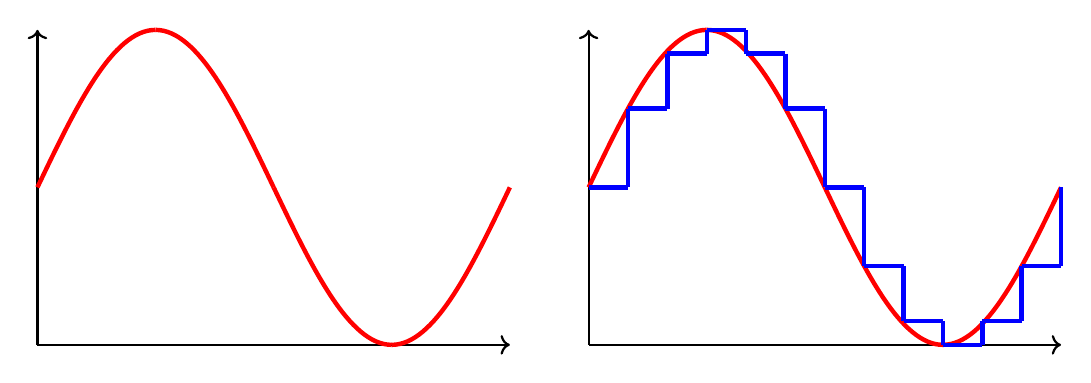
\begin{tikzpicture} 
 %%Denne første modellen er input signalet
    % We start by drawing the diagram:
    \draw [thick, ->] (0,0)--(6,0);
    \draw [thick, ->] (0,0)--(0,4);
    \draw[ultra thick, red] (0,2) sin (1.5,4);
    \draw[ultra thick, red] (1.5,4) cos (3,2);
    \draw[ultra thick, red] (3,2) sin (4.5,0);
    \draw[ultra thick, red] (4.5,0) cos (6,2);
  
  %% Denne andre modellen er samplet signal
    % We start by drawing the diagram:
    \draw [thick, ->] (7,0)--(13,0);
    \draw [thick, ->] (7,0)--(7,4);
    \draw[ultra thick, red] (7,2) sin (8.5,4);
    \draw[ultra thick, red] (8.5,4) cos (10,2);
    \draw[ultra thick, red] (10,2) sin (11.5,0);
    \draw[ultra thick, red] (11.5,0) cos (13,2);

    \draw[ultra thick, blue] (7,2) -- (7.5,2);
    \draw[ultra thick, blue] (7.5,2) -- (7.5,3);
    \draw[ultra thick, blue] (7.5,3) -- (8,3);
    \draw[ultra thick, blue] (8,3) -- (8,3.7);
    \draw[ultra thick, blue] (8,3.7) -- (8.5,3.7);
    \draw[ultra thick, blue] (8.5,3.7) -- (8.5,4);
    \draw[ultra thick, blue] (8.5,4) -- (9,4);
    \draw[ultra thick, blue] (9,4) -- (9,3.7);
    \draw[ultra thick, blue] (9,3.7) -- (9.5,3.7);
    \draw[ultra thick, blue] (9.5,3.7) -- (9.5,3);
    \draw[ultra thick, blue] (9.5,3) -- (9.5,3);
    \draw[ultra thick, blue] (9.5,3) -- (10,3);
    \draw[ultra thick, blue] (10,3) -- (10,2);
    
    \draw[ultra thick, blue] (10,2) -- (10.5,2);
    \draw[ultra thick, blue] (10.5,2) -- (10.5,1);
    \draw[ultra thick, blue] (10.5,1) -- (11,1);
    \draw[ultra thick, blue] (11,1) -- (11,0.3);
    \draw[ultra thick, blue] (11,0.3) -- (11.5,0.3);
    \draw[ultra thick, blue] (11.5,0.3) -- (11.5,0);
    \draw[ultra thick, blue] (11.5,0) -- (12,0);
    \draw[ultra thick, blue] (12,0) -- (12,0.3);
    \draw[ultra thick, blue] (12,0.3) -- (12.5,0.3);
    \draw[ultra thick, blue] (12.5,0.3) -- (12.5,1);
    \draw[ultra thick, blue] (12.5,1) -- (13,1);
    \draw[ultra thick, blue] (13,1) -- (13,2);
  \end{tikzpicture}\caption{Input signal and sampled signal} \label{sample:hold}
\end{figure}


\begin{figure}
\begin{center}
\begin{circuitikz}
\draw (0,0) node[anchor=east]{$v_{in}$}[o-] -- (1,0);
\draw (1,0) to[push button, l=$\phi_{1}$] (3,0);
\draw (3,0) to[C, l=$C$] (3,-2) node[ground] {};
\draw (3,0) -- (5,0)node[anchor=west]{$v_{out}$}[-o];
\end{circuitikz}\caption{Sample and Hold} \label{sample:hold:2}
\end{center}
\end{figure}


\subsubsection{Comparator}
\subsubsection{Digital-to-analog converter}
\subsubsection{Logic}
\
\subsection{Requirements}
In todays technologies, it is importatint to consume as low power as possible, and be as fast as possible. Due to this, we are going to design a SAR ADC which are capable 
of running with a powersupply of 1.2 V and have sampling frequency of 1 MHz. The overall requirements are listed bellow.\\
\textbf{SAR ADC}
\begin{itemize}
 \item Input sampling rate: 1 M samples/s
 \item Output resolution: 8 bits
 \item Supply voltage: $V_{DD} = 1.2 V$, and $V_{SS} = 0 V$
 \item No missing codes
 \item Monotonic
\end{itemize}
\textbf{DAC}
\begin{itemize}
 \item Sampling rate: 8 M samples/s
 \item Resolution: 8 bits
 \item Supply voltage: $V_{DD} = 1.2 V$, and $V_{SS} = 0 V$
 \item DNL < $\pm$ 0.5 LSB
 \item INL < $\pm$ 0.5 LSB
 \item $V_{OUT(P\_P)} \geq 0.6$
 \item $C_{load} = 50 fF$
\end{itemize}
\textbf{Comparator}
\begin{itemize}
 \item 
\end{itemize}


Critical parts in SAR ADCs 
\begin{itemize}
 \item Comparator
 \item DAC
\end{itemize}
SAR ADCs limitations:
\begin{itemize}
 \item The settling time is the DAC, whick must settle within the resolution of the overall converterm for example, 1/2 LSB (Least significant bit)
 \item The comparator, which must resolve small differences in $V_{in}$ and $V_{DAC}$ within the specified time
 \item The logic overhead
\end{itemize}
Comparator:
\begin{itemize}
 \item The comparator does not effect the overall linearity 
\end{itemize}

%-----------Background-------
\chapter{Background}


%-----------Main part--------          
\chapter{Planning the project} 
\section{Task 1}
\subsection{Task 1.B}
\begin{table}
 \centering
 \caption{Comparation of different ADCs}
 \label{comp:adc}
 \begin{tabular}{|l|l|l|l|l|}
 \hline
                  & SAR        & Flash   & Sigma-Delta  & Integrating                      \\ \hline
 Conversion speed & Low-medium & Fast    & Low          & Depending on \\
		  &	       &	 &		&reolution and clock 		   \\ \hline
 Sampling rate    & Nyquist    & Nyquist & Oversampling & Nyquist                          \\ \hline
 Area             & Low        & High    & Medium       &                                  \\ \hline
 \end{tabular}
 \end{table}



%-----------Results----------
\chapter{Results} 
\chapter{Discussion and conclusion}
\section{Discussion}
\subsection{Proposal of improvement}
\section{Conclusion}

% \backmatter{}


\begin{appendices}
\chapter{Software and instrument overview}
\end{appendices}

\printbibliography{}

\end{document}


% --------------------------------------------------------------------
% Fotnote eksempel
% Hei \footnote{\url{http://www.google.fi/}}
% --------------------------------------------------------------------
% Figur eksempel
% \begin{figure}[!ht]
%   \centering
%     \includegraphics[width=0.5\textwidth]{filplassering}
%     \caption{Bildetekst}
%     \label{fig:}
% \end{figure}
% ---------------------------------------------------------------------
% For en mer bestemt plassering:
% 
% \begin{wrapfigure}{r}{0.5\textwidth}
%   \begin{center}
%     \includegraphics[width=0.48\textwidth]{filplassering}
%   \end{center}
%   \caption{Bildetekst}
%   \label{fig:}
% \end{wrapfigure}
% 
% Plasseringer for bilde:
% r 	R 	right side of the text
% l 	L 	left side of the text
% i 	I 	inside edge–near the binding (in a twoside document)
% o 	O 	outside edge–far from the binding
% ----------------------------------------------------------------------
% For å innkludere skjematiske tegninger:
%
%\begin{circuitikz}[scale=1.25]

% \draw (-1,0) node[anchor=east] {} to [short, *-*] (1,0);
% \draw (-1,2) node[anchor=east] {} to [inductor, *-*,  l=$\Delta x L$] (1,2);
% \draw (-1,0) to [open, l=$\cdots$] (-1,2);    
% \draw (3, 0) to (1, 0) to [capacitor, l=$\Delta x C$, *-*] (1, 2) to [inductor, *-*, l=$\Delta x L$] (3, 2);
% \draw (5, 0) to (3, 0) to [capacitor, l=$\Delta x C$, *-*] (3, 2) to [inductor, *-*, l=$\Delta x L$] (5, 2);
% \draw (7, 0) to (5, 0) to [capacitor, l=$\Delta x C$, *-*] (5, 2) to [inductor, *-*, l=$\Delta x L$] (7, 2);
% \draw (9, 0) to (7, 0) to [capacitor, l=$\Delta x C$, *-*] (7, 2) to [inductor, *-*, l=$\Delta x L$] (9, 2);
% \draw (9,0) node[anchor=east] {} to [short, *-*] (9,0);
% \draw (10,0) to [open, l=$\cdots$] (10,2);

% \end{circuitikz}
% ----------------------------------------------------------------------
% Paranteser
% 
% \big( \Big( \bigg( \Bigg( 	
% \big] \Big] \bigg] \Bigg] 	
% \big\{ \Big\{ \bigg\{ \Bigg\{ 	
% \big \langle \Big \langle \bigg \langle \Bigg \langle 	
% \big \rangle \Big \rangle \bigg \rangle \Bigg \rangle 	
% -----------------------------------------------------------------------
